% 14:27 09/04/2023
\chapter{System Design}
% Provide a detailed explanation of the overall system architecture
% \cite{lin1991divergence}, i.e. the HOW of the project.
% Use UML, system architecture diagrams, screenshots, code snippets 
% and algorithms to illustrate your design.

This chapter features a discussion on how the project was designed
and on the design decisions used throughout.
Diagrams and screenshots of the various components will be provided
and so will implementation snippets of code.

\begin{figure}[h!]
    \centering
    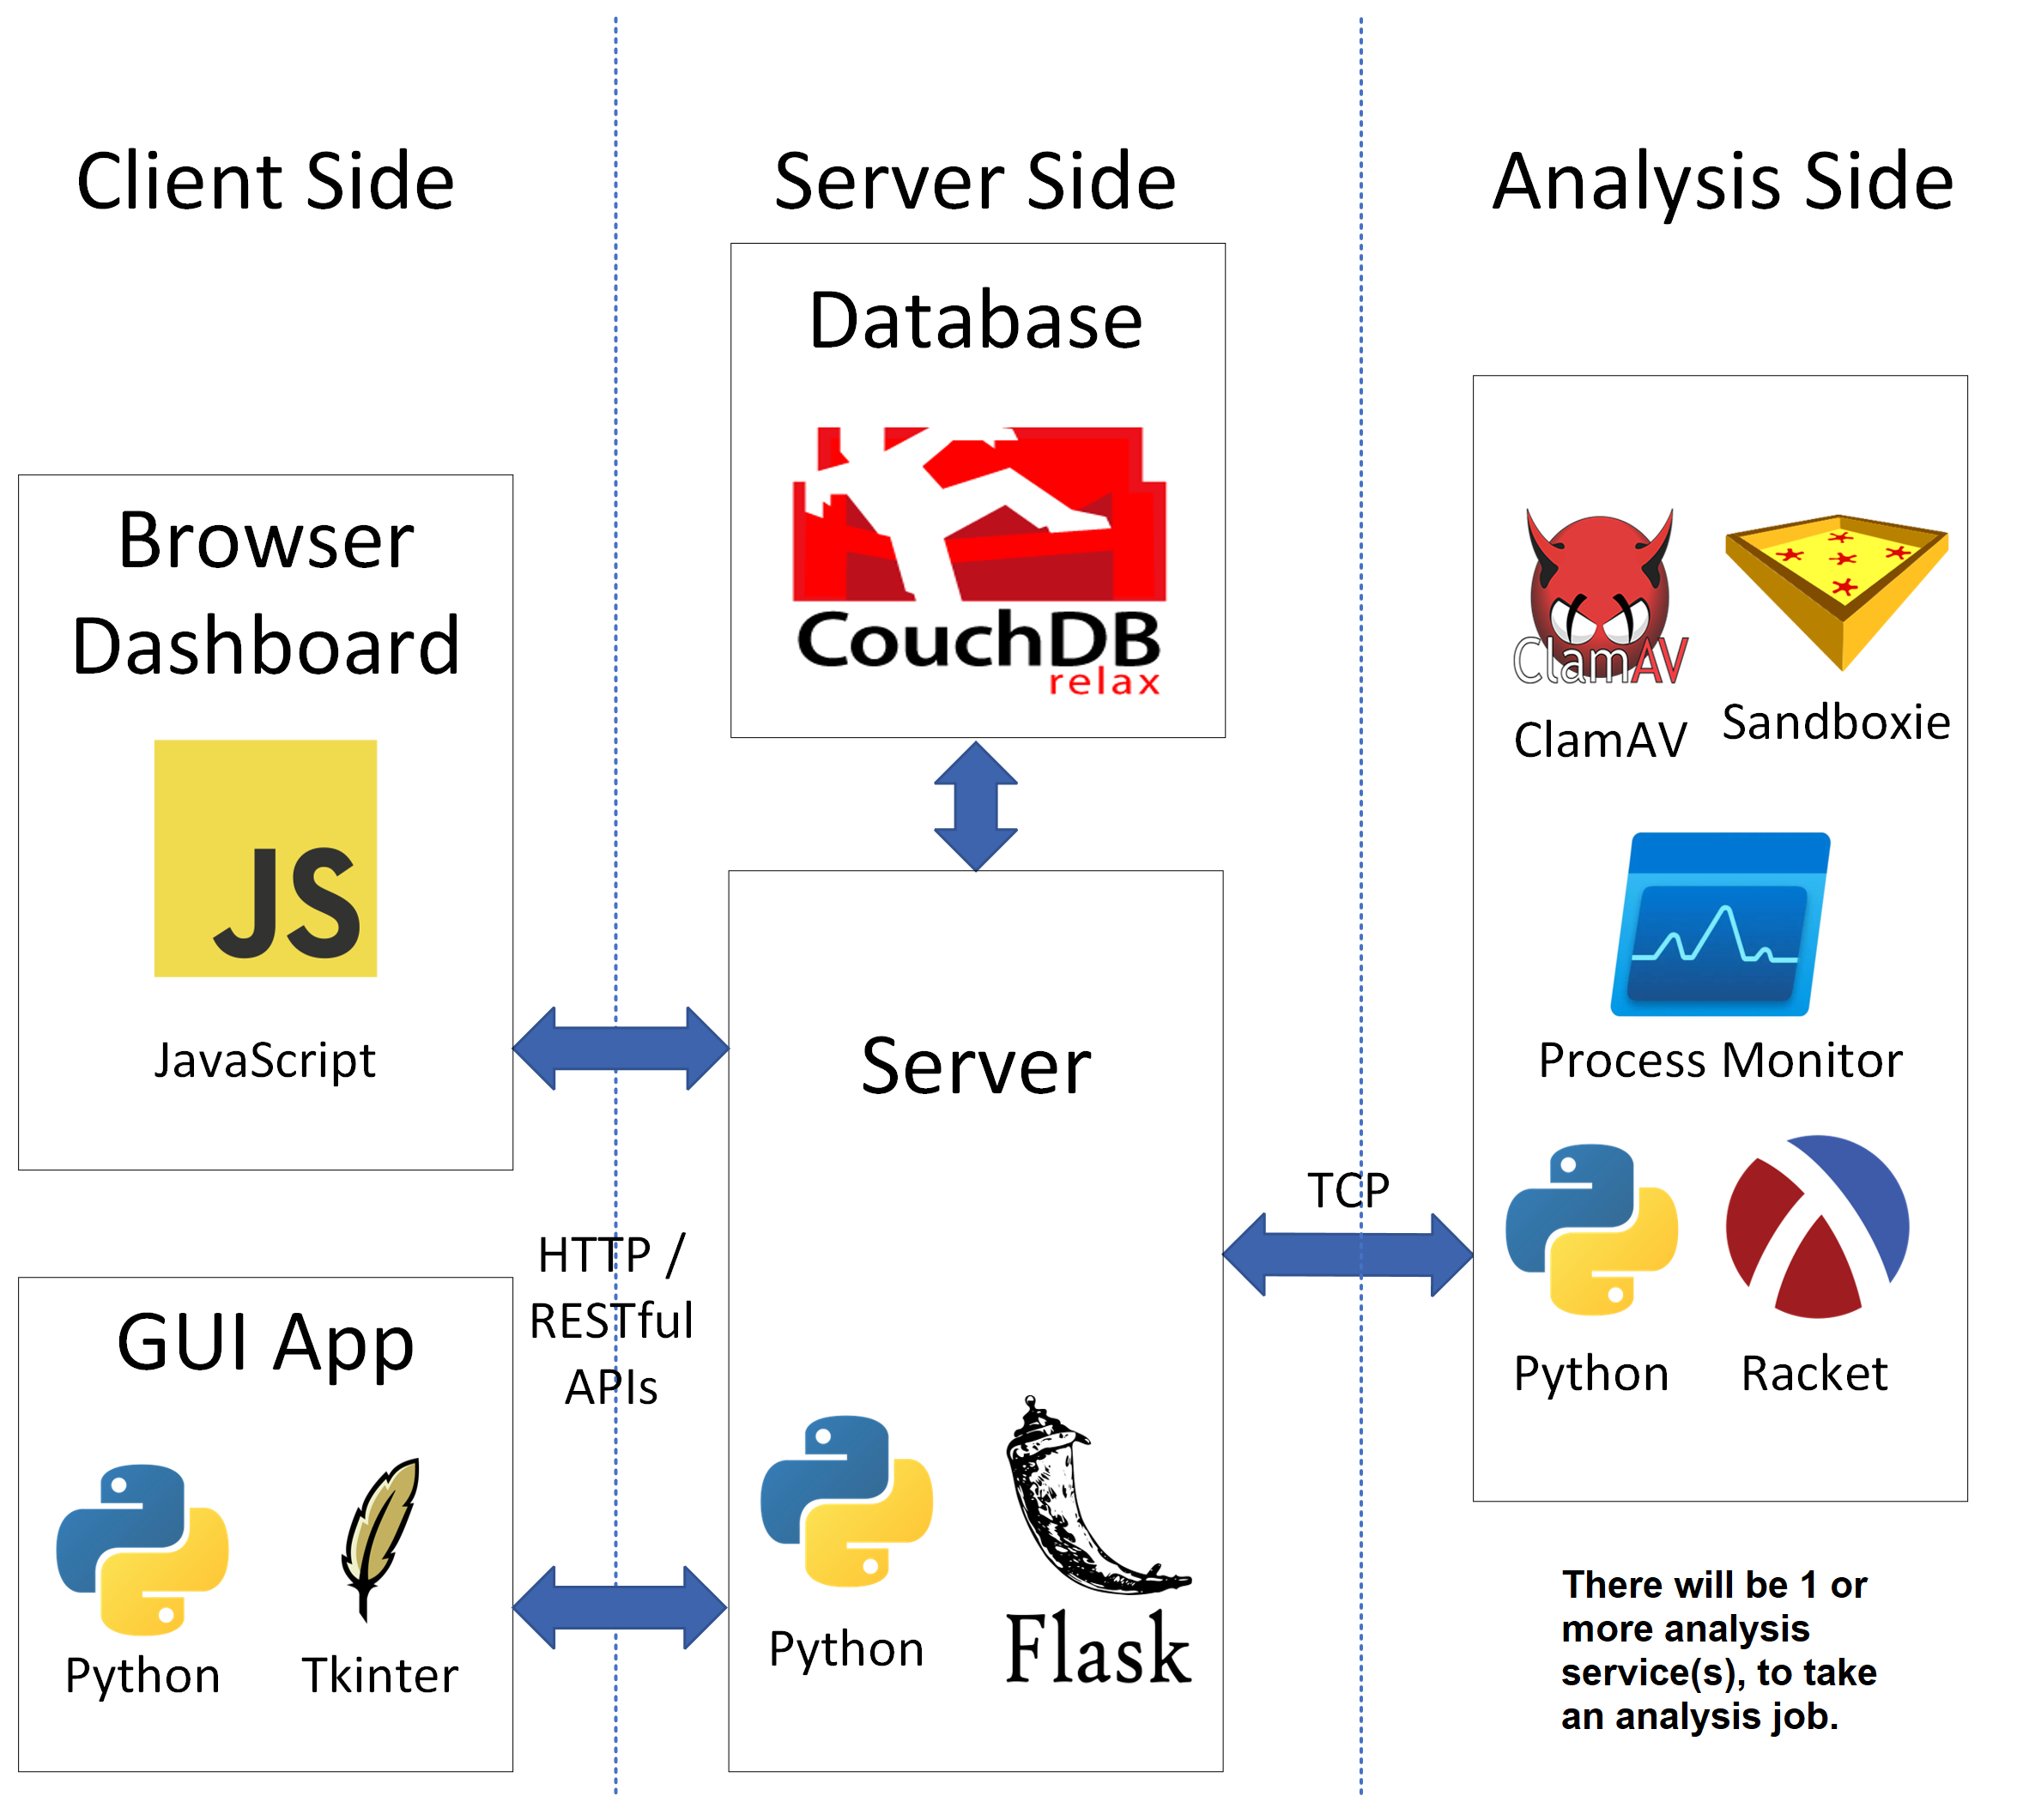
\includegraphics[width=0.75\textwidth]{images/diagrams/architecture}
    \caption{System Architecture Diagram}
    \label{image:sysArchitecture}
\end{figure}

The system architecture diagram shown above provides
a top-down view of the platform during execution.

It can be divided into three sections,
each with the ability to run on different computers.

On the left side, there is the client software,
which includes the GUI application and the dashboard
that runs in the administrator's browser.
In the middle, there is the server. On the right side,
there are instances of the sandbox analysis workers.
Multiple instances of these workers can be created.

\section{Windows GUI Application}
The GUI application runs on a user's computer
and it runs on the client side

Python files with the \texttt{frame.py} suffix contain Tkinter frame classes,
and each of these files contains only one class that inherits the Tkinter \texttt{Frame} class.

This allows all code related to that frame, to be fully encapsulated,
for instance in the \texttt{PreferencesFrame}, the buttons for changing the settings
are kept inside the class and not accessible to other classes.

The main code of the application can be found in the
\texttt{client/src/\_\_main\_\_.py} file,
the purpose of this file is to setup up the Tkinter window and run the main loop of execution.

In order for the application to do anything with the server,
it first needs to be provisioned.
The requirement of provisioning prevents unauthorised
clients from executing tasks on the workers.

Administrators can optionally enable auto-provisioning on the server,
allowing clients to provision without manual intervention,
manual intervention requires administrators to issue users with a token,
and users will input this token into their application on the first load.

\subsection{User Interface}
The client post-provisioning features a Tkinter \texttt{Notebook},
with 3 sub-frames, \textbf{Main Page ("Caladium")},
\textbf{Quarantine} and \textbf{Preferences}.
You can navigate through these by clicking on each label on the window.
The \texttt{Notebook} Tkinter widget allows you to
group frames together allowing navigation between them.

The Main Page in the frame features a button to manually scan a file,
and a label indicating the current scanning directory.

\subsubsection{Quarantine Page}
The code for the quarantine page can be found in
\texttt{client/src/quarantineframe.py}.

The quarantine frame displays all the files currently in quarantine,
it shows the original location of each file,
with the ability to restore each file,
by clicking on the entry in the list box
and then pressing the "Restore file" button.

A screenshot of the quarantine page can be seen below,
you can also see the menu bar at the top,
showing how you can switch between each frame.

\begin{figure}[h!]
    \centering
    \label{image:quarantinePageScreenshot}
    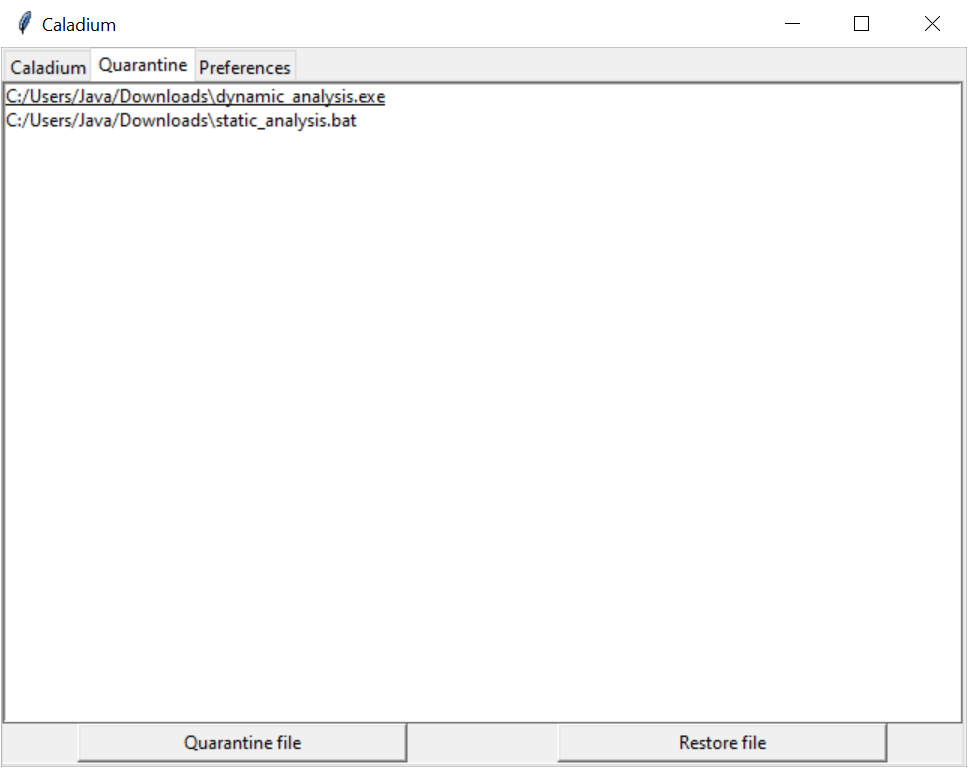
\includegraphics[width=0.75\textwidth]{../docs/client.png}
    \caption{Quarantine Page Screenshot}
\end{figure}

To add files to the quarantine users can press the "Quarantine file" button,
and then select the file in the file picker.

To allow users to pick files from their computers, \\
I'm using \texttt{tkinter.filedialog.askopenfile("rb")},
which returns a handle to a file when picked.

\subsubsection{Preferences Page}
The preferences page contains buttons,
allowing users to adjust settings.

The "Uninstall Caladium" button will uninstall Caladium from your computer,
it does this by dropping a script into your \texttt{\%TEMP\%} directory,
the client will close, and shortly afterwards the script will execute.
It will then delete the Caladium directory from the \texttt{Program Files} directory,
and cleans up the shortcuts on the desktop and the startup directory.

Pressing the "Change Scanning Directory" button will open a directory picker,
similar to the file picker shown above in the quarantine frame.
Once the user has selected the new directory,
it will change the current scanning directory to the one selected,
and update the label on the main page to reflect this.

"Unprovision Caladium" will reverse the provisioning,
and will close the application. When the user reopens
the application, they will be prompted to re-provision.

\subsubsection{Scanning Frame}
The code that implements the scanning frame can
be found in \texttt{client/src/scanningframe.py}.

When the scanning process begins, this window will open,
it will have a text box containing real-time feedback from the server,
and at the bottom will have a progress bar.

The progress bar is implemented using the \texttt{tkinter.tk.Progressbar} widget,
the state of the bar is updated using its \texttt{value} attribute. 

\begin{figure}[h!]
    \centering
    \label{image:scanningFrameScreenshot}
    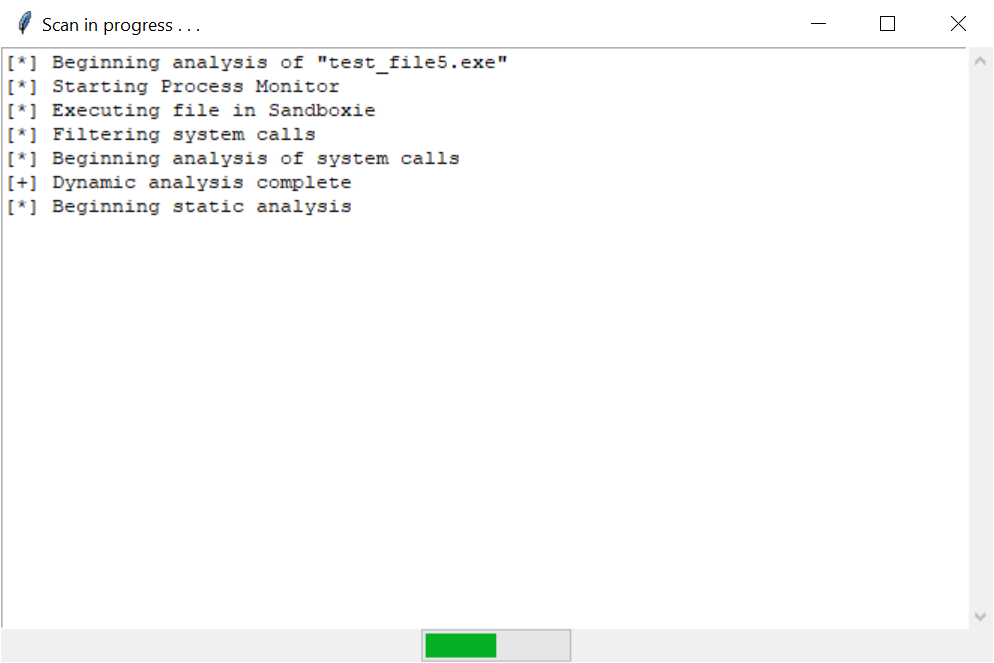
\includegraphics[width=0.75\textwidth]{images/screenshots/scanning_frame}
    \caption{Scanning Frame Screenshot}
\end{figure}

In the screenshot above, you can see the log messages coming back from the server,
each message is prefixed with an error level indicator, \texttt{[+]} meaning success
and \texttt{[-]} meaning failure.

At the bottom, you can see the current progress stage,
in this case, its \texttt{50\%}.

\subsection{Quarantine}
When files are added to the quarantine,
they are encrypted with an XOR cipher to avoid accidental
execution of malware in the event that the user
accidentally stumbles upon the location of the quarantine.

This is a snippet of the code from \texttt{client/src/quarantine.py};
it takes in input file data and its key and applies the XOR of the key to each byte,
then returns the newly encrypted version.

\begin{lstlisting}
def _xor_bytes(self, data_bytes, xor_key_bytes):
    # Convert bytes to list of ints
    data_bytes = [i for i in data_bytes]

    # XOR each one with the xor key
    for i in range(len(data_bytes)):
        data_bytes[i] ^= xor_key_bytes[i % len(xor_key_bytes)]

    return bytes(data_bytes)
\end{lstlisting}

\subsection{Directory Scanning}
The client has the ability to identify newly downloaded files,
this is implemented in \texttt{client/src/dirchangelistener.py}.
This functionality is achieved by scanning for new files in a directory.

This is implemented in a class called \texttt{DirChangeListener},
an instance of this class will be made, and will be passed a callback function,
that will be called when a new file appears in the directory.

A \textbf{tkthread} thread is spawned which loops
and checks for new files on every iteration.
The current directory state is obtained using
\texttt{os.listdir(dir\_name)} and compared with the last state.
To prevent the application from locking up,
the Tkinter GUI is given some time to render on each iteration.
This is explained in detail in the technology review chapter.

\section{Server Dashboard}
The dashboard is a single-page web application (SPA)
and is fully written in JavaScript.
This means when you navigate to another page in the dashboard
it doesn't have to pull it from the server,
just fetch the data specific to that page,
then renders it dynamically using JavaScript.

Below you will find a screenshot of the dashboard's index page,
the dashboard lists all the sub-pages.

The \texttt{Clients}, \texttt{Patterns}, \texttt{Tasks} and \texttt{Workers} are all
list pages, containing a list of records for that table.

The index page shows a statistical chart for each,
the bar chart shown in green shows the distribution of records for each month,
in this case, it only shows March.

Clicking on any of the titles on the index page will bring you to its list page.

\begin{figure}[h!]
    \centering
    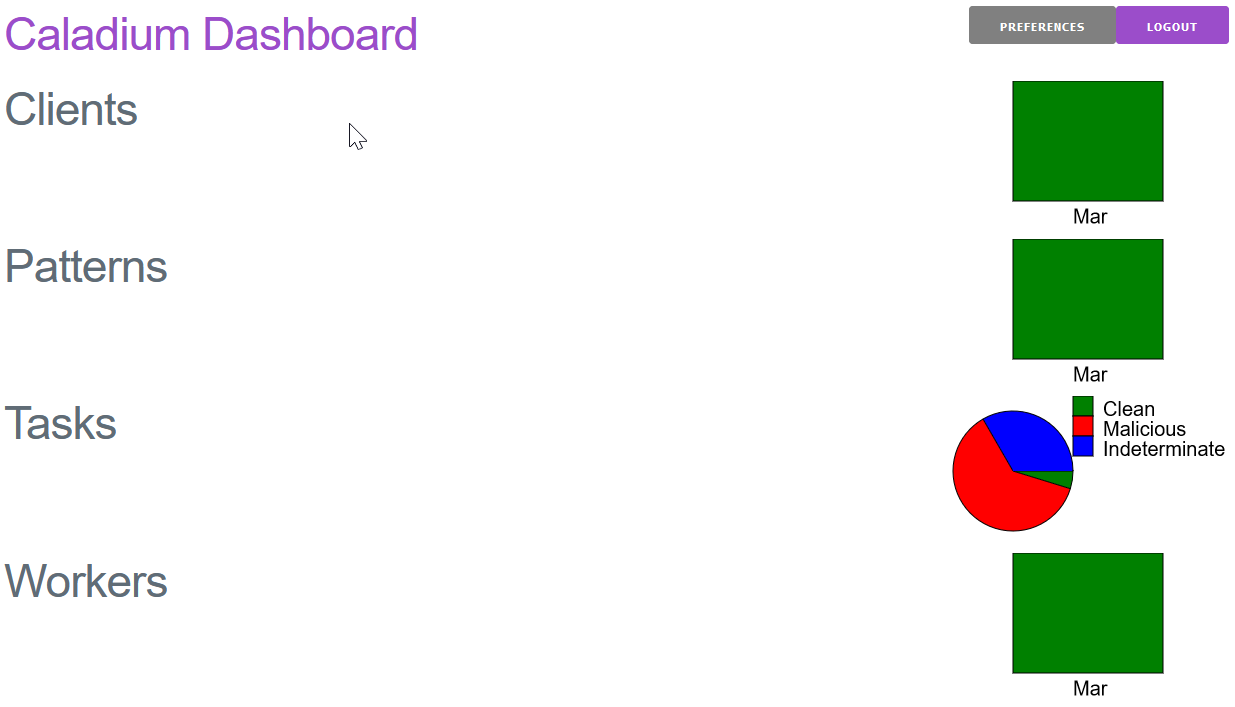
\includegraphics[width=0.75\textwidth]{../docs/dashboard.png}
    \caption{Dashboard Index Screenshot}
    \label{image:dashboardScreenshot}
\end{figure}

\subsection{Single-Page Application}
A single-page application can update its contents
without having to refresh the page,
using JavaScript to dynamically fetch content from an API.
\cite{jadhav2015single}
For example, in my dashboard, when a user clicks on a button,
content such as a list of workers
will be fetched from an API and then displayed on the screen.

Upon loading a new page, the contents of the page are
dynamically generated using DOM Lisp expressions.
The URL of the page is then updated using the History API.

In the \textbf{server/static/js/index.js} I have a dictionary called
\textbf{routes} containing a list of all
the routes and their corresponding
page classes and their page titles.
When a page is loaded,
the routes dictionary is queried using the current URL in the browser,
and the corresponding page class is then loaded.

Below you can find a code snippet of the routes found in \texttt{index.js},
for example, the "/" route, will load the \texttt{IndexPage} class,
and sets the title to "Dashboard".
\begin{lstlisting}
// These are all the defined pages
const routes = {
    "/": {
        "body": IndexPage, "title": "Dashboard"
    },
    "/clients": {
        "body": ClientsPage, "title": "Clients"
    },
    "/login": {
        "body": LoginPage, "title": "Login"
    },
...
\end{lstlisting}

\subsection {Page Class Hierarchy}
The dashboard is object-oriented,
all of the main code can be found in
the \textbf{server/static/js/index.js} file.
This contains code for communicating with
the server endpoints and the classes for each page.

Below you can find a diagram showing the hierarchy of the classes,
all classes inherit from the \texttt{Page} class,
as they share common functionality,
this also upholds the DRY principle.

\begin{figure}[h!]
    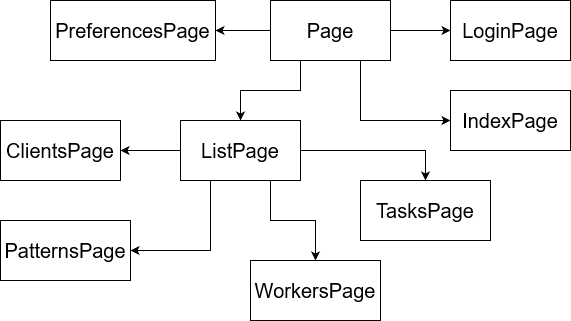
\includegraphics[width=0.9\textwidth]{images/diagrams/dashboard_hierarchy.drawio}
    \caption{Page Class Hierarchy Diagram}
    \label{image:sysArchitecture}
\end{figure}

Each page class must implement the \textbf{loadPage} method,
which is called when the page is loaded.
This function pulls data from the server,
that is specific to that page.

\subsection{DOM Lisp Expressions}
In a single-page application (SPA), all page content
is dynamically generated without
needing to pull HTML from a server when navigating between pages.

Initially, I considered embedding raw HTML within the JavaScript code,
but found it to be inelegant.
As a solution, I created a domain-specific language (DSL)
to represent the Document Object Model (DOM) as Lisp expressions.

My approach involved storing these Lisp expressions as strings within each page class,
they can include parameters which could be replaced
with their actual values during page loading.
This approach allowed me to encapsulate the expressions within each page class.

This approach simplifies the creation of the visual components of each class.
I developed a library, that can be found at \textbf{server/src/static/js/pantothenic.js},
which has a \textbf{generateDOM} function that takes a
DOM Lisp expression and its parameters, and returns a DOM object.

The DOM is a tree of nested elements that represents a web page's HTML.
By using Lisp expressions as a DSL to represent DOMs,
I have created a more elegant solution for generating dynamic
content without embedding ugly HTML.

Below you will find an example of a DOM Lisp expression.
This is taken from the \textbf{Preferences} class in the
\textbf{server/src/static/js/index.js} file.
It describes the HTML components for that page,
it includes an input box for a new password for the admin user
and a button that toggles the auto-provisioning of new users.
When the user clicks the button, it calls the
\textbf{toggleAutoProvision} method within the class.

The navigation bar is also represented as a DOM expression,
this can be found in the main \texttt{Page} class,
that all pages inherit.
This avoids repeating myself, allowing easy maintenance.

The \texttt{navigationBar} parameter found below,
is replaced with the actual navigation bar when loaded.

\begin{lstlisting}
this.body = ` (div (hash "children"
                (list
                    navigationBar
                    (input (hash "type" "password" "id"
                        "newPassword" "placeholder" "New Password"))
                    (button (hash "onclick" changePasswordOnClick
                        "innerHTML" "Update Password"))
                    (hr)
                    (button (hash "onclick" toggleAutoProvision
                        "innerHTML" autoProvisionButtonText)))))`;
\end{lstlisting}

\subsection{Login Page}
\begin{figure}[h!]
    \centering
    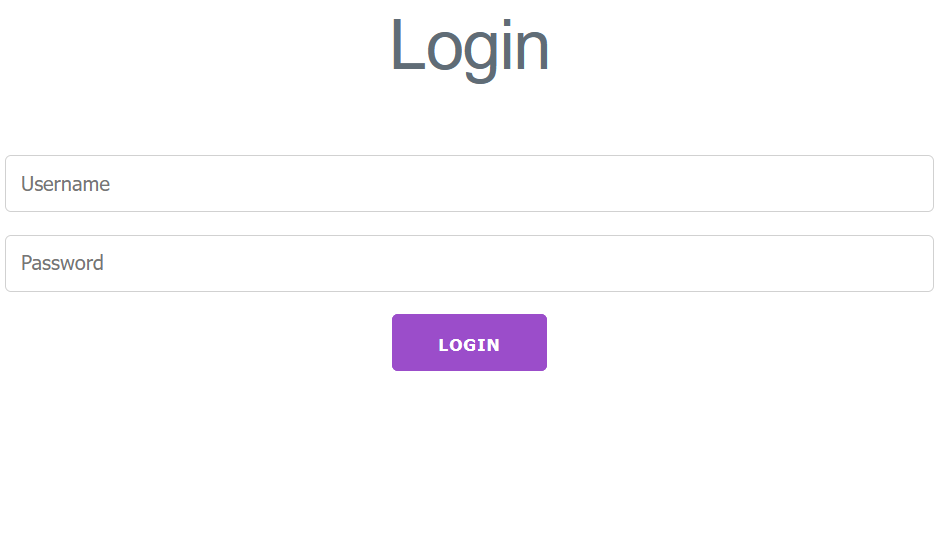
\includegraphics[width=0.75\textwidth]{images/screenshots/login_page}
    \caption{Login Page Screenshot}
    \label{image:loginPageScreenshot}
\end{figure}

Before you are able to perform any actions,
you must log in to the dashboard,
using the Login page as shown above,
the default username and password are "root" and "root".

These can be changed on the preferences page once logged in,
the password is hashed with SHA-256, so its
the plain-text version cannot be retrieved in the event of a compromise.

Input these details into the username and password fields
and press "Login" as seen in the screenshot above.

\subsection{List Page}
Below you can find an example screenshot of one of the list pages,
the "Clients" page list all the clients in the client's table,
each list page has a button at the top allowing you to delete all the records.

Each record has a number of buttons that can perform actions on that record,
these are specified by the class that inherits the list page class.

\begin{figure}[h!]
    \centering
    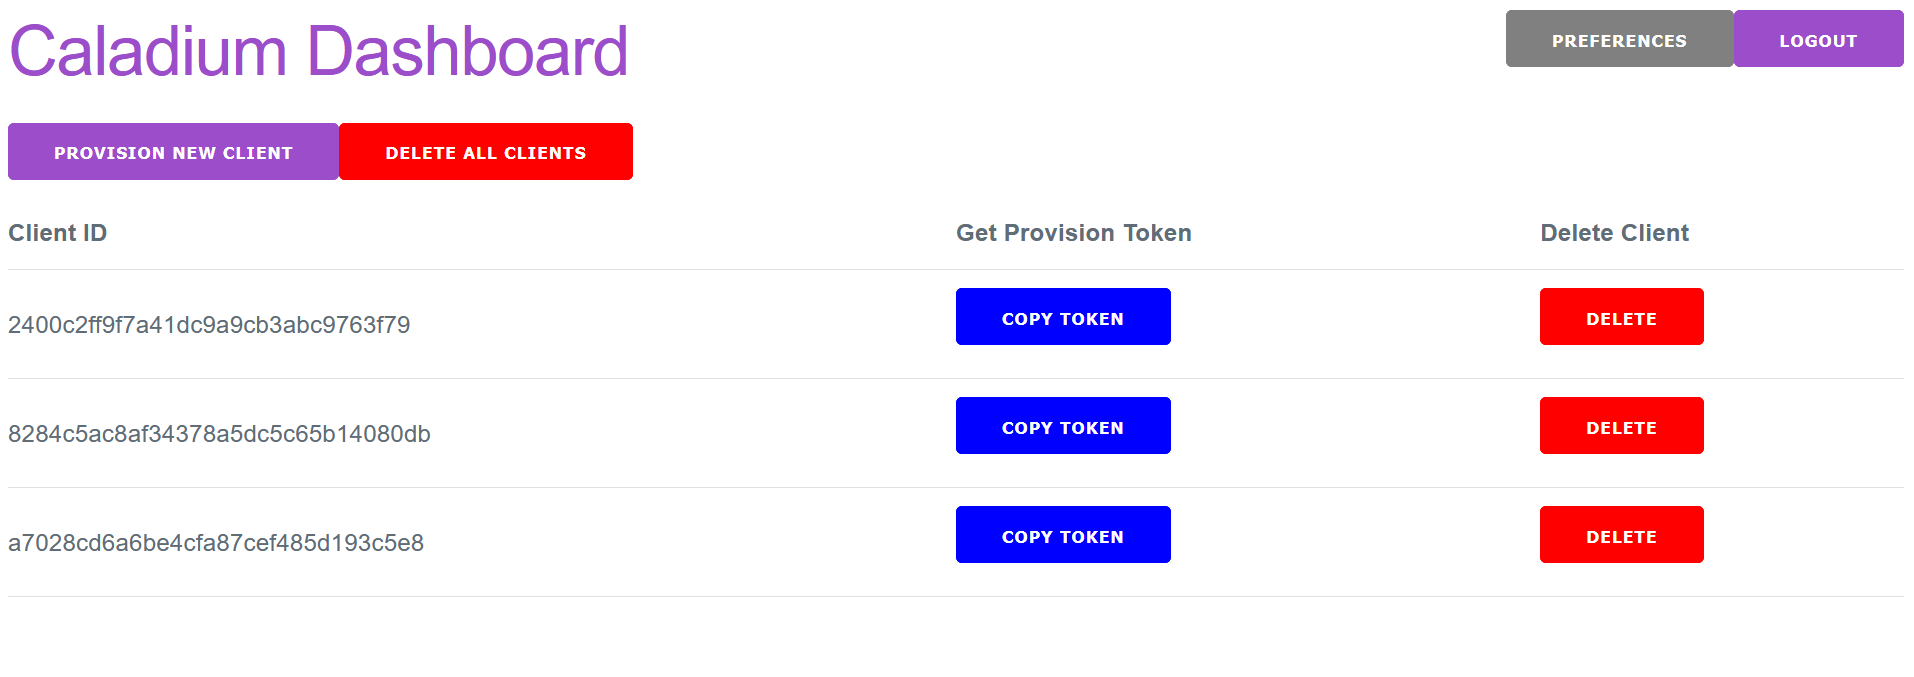
\includegraphics[width=0.9\textwidth]{images/screenshots/list_page}
    \caption{List Page Screenshot}
    \label{image:listPageScreenshot}
\end{figure}

\section{Server Side}
The server bridges communications between the clients and sandbox instances.
Clients use HTTP to perform actions on the server.
I'm using Flask on the server to facilitate this.
The server also needs to be able to persist data,
which will be done with CouchDB.
Below, I will show how I abstracted the table
records into a class called \texttt{DatabaseRecord}.

\subsection{Server Endpoints}
The server uses the Flask micro-framework to provide the RESTful API.
I decided to categorise the API into four sections:
clients, patterns, tasks and workers.
Flask supports a feature called blueprints,
which allows you to split your web application into multiple components.
I used a blueprint for each of the four sections of the API,
and each blueprint is stored in a separate file
with the name of the API resource.

This is an example of a blueprint taken from the worker's blueprint.
\begin{lstlisting}[language=python]
...

import flask

...

workers = flask.Blueprint(__name__, "workers")

@workers.get("/api/workers")
def get_records_route():
    return database.get_caladium_collection("workers")

...
\end{lstlisting}

Each of the endpoints is RESTful the HTTP method name signifies
the type of operation to be performed on that resource,
the table below will show each method used in the server
and a description of its purpose.

\begin{table}
    \centering
    \begin{tabular}{|p{2cm}|p{6cm}|}
        \hline
        \multicolumn{2}{|c|}{HTTP Methods and Descriptions} \\
        \hline
        Method & Description \\
        \hline
        GET & Fetches data from a server, without modifying it. \\
        \hline
        POST & Creates new data on the server. \\
        \hline
        DELETE & Delete a record by ID. \\
        \hline
    \end{tabular}
    \caption{HTTP Methods and Descriptions}
    \label{table:httpMethods}
\end{table}

\subsection{Database}
Data was persisted using CouchDB,
and the server communicates with it using the pycouchdb module.

Having to write out the pycouchdb queries became cumbersome,
so I decided to abstract the records of the database away using a class called
\texttt{DatabaseRecord}, this can be found in \texttt{server/src/database.py}.

Now If I wanted to fetch a record from a table I would do this:
\begin{lstlisting}
task_record = database.get(TaskRecord, task_id)
\end{lstlisting}

To get/set attributes of the record,
I would use the instance methods of \texttt{DatabaseRecord}.

In the case of the setting operations,
the \textt{DatabaseRecord} class would push the modified attribute
of the record to the CouchDB instance.

\begin{lstlisting}
print("This is worker ID:", task_record.get("worker_id"))

# Setting new worker_id
task_record.set("worker_id", "1")
\end{lstlisting}

\subsection{Authentication}
Before processing each call in the server,
the \texttt{before\_request} function is called,
as seen in the \texttt{\_\_main\_\_.py} file.
It checks the token contained in the request and
verifies if the caller has the required permissions to execute the request.

\subsection{Cloud Hosting}
I'm using Microsoft Azure to host a Linux server in the cloud.
During development, to test the latest version,
I would git pull the latest version of the repository and
then build and run the Docker image using the \texttt{Dockerfile}.

I am also using Azure to host the CaladiumBot server part.
To expose ports other than 80,
which is the default for HTTP web traffic,
I had to manually add the ports in the Azure dashboard.

My promotional page, which is hosted on GitHub Pages,
communicates with this CaladiumBot server.
But could only do this if the server had a valid HTTPS certificate.
To get an HTTPS certificate you need your server to
be linked with a domain name.
So I purchased a domain name, and generated an HTTPS certificate,
then I succeeded in getting it working.

\section{Analysis Side}
The main file of the analysis side can be found in
\texttt{sandbox/src/main.rkt},
it is written in the Racket language,
when it begins it will open a TCP port,
ready to accept incoming requests

\subsection{Communication with Server Side}
When a client asks the server to analyse a file,
the server needs to assign the job to one of its worker instances.
To keep track of what the workers are doing,
the server needs a way to communicate with them in real time.
I chose to use TCP for this purpose,
a communication method that allows data to be sent and received between devices.

The main program for analysing the file is written in Racket,
which has built-in support for TCP.

The server is written entirely in Python,
which also supports TCP using the sockets library.
But, I encountered a problem when trying to receive information from the workers.
The server had no way of knowing how much data was being sent,
so I looked for a solution and found a
helpful answer on Stack Overflow \cite{chqrlie:2022}
The solution was to include the length of the incoming
data at the beginning of the packet
so that the server would know how much data to expect.

This code can be found in \texttt{sandbox/src/caladium\_resp.py}.
It initially sends the size of the data,
it uses the struct module to convert the Python integer,
into bytes form, and the > denotes that it will be in big-endian.
(most significant byte on the left).
Then sends the actual data,
the other computer listens for the initial size,
then knows how much to read.

\begin{lstlisting}
output_func(struct.pack(">I", len(json_obj_bytes)))
output_func(json_obj_bytes)
\end{lstlisting}

\subsection{Scanning Process}
When a file is passed to the analysis worker from the server,
the scanning process begins as seen in diagram \ref{image:scanningProcess}.
Malicious patterns are also passed to the worker
alongside the file to be scanned.

\begin{figure}[h!]
    \centering
    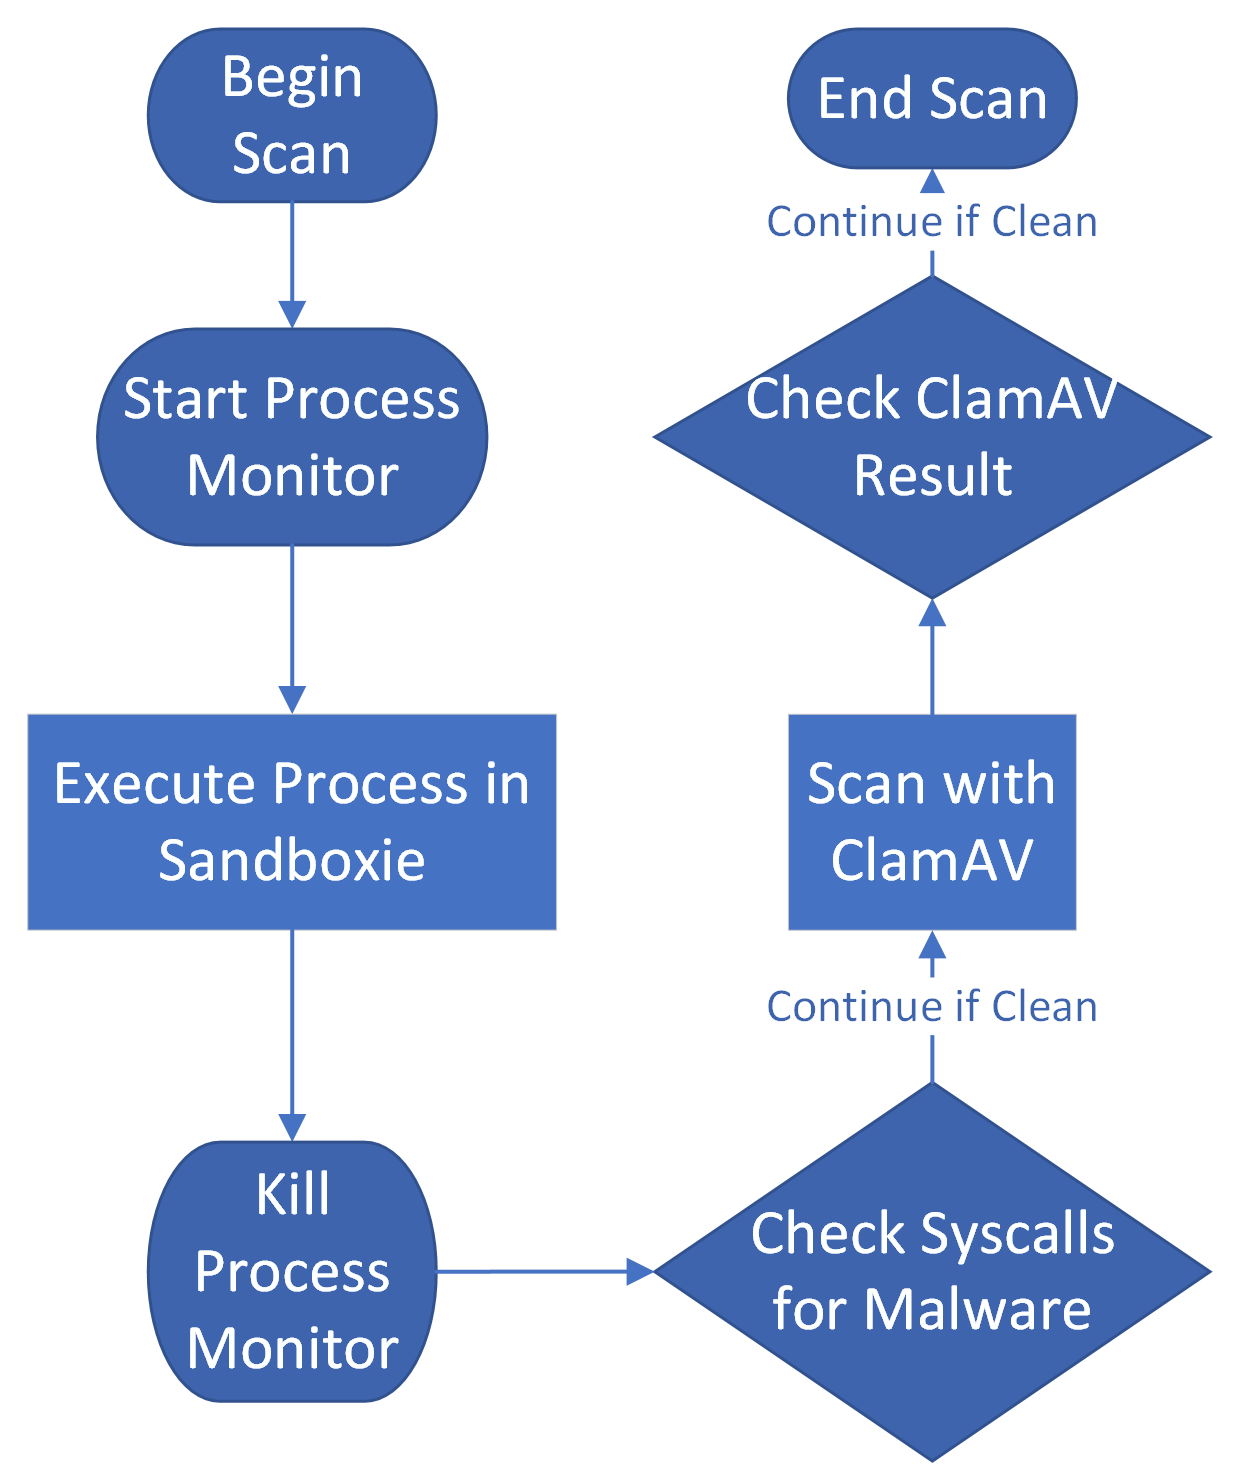
\includegraphics[width=0.5\textwidth]{images/diagrams/scan_process}
    \caption{Scanning Process Diagram}
    \label{image:scanningProcess}
\end{figure}

The first part of the process is dynamic analysis.
It begins by spawning Process Monitor,
then the target file is executed in Sandboxie.
While this is happening,
Process Monitor is logging the system calls performed by the target file.
Once the process is finished or a certain amount of time elapses (timeout),
Process Monitor is killed. This will return a list of system calls in CSV format.

Then it must iterate through all these system calls,
to see if there is a match with one of the patterns
that was passed to the worker.
If there isn't a match, it will continue to the next stage of the process,
the static analysis.

This is done with ClamAV,
which passes the location of the file to
\texttt{clamscan.exe} as a parameter.
It will check the output of this to see if it's malicious.
If both strategies detect nothing,
the scan will end and the file can be deemed clean.
Each state of the process gives updates back to the server along with
text messages that will be presented to the client.

\section{Promotional Page}
In addition to the sub-projects above, the platform
features a promotional page hosted on GitHub Pages.

It contains two buttons on the top of the page,
the first downloads the latest build of the
Caladium client from the GitHub releases.

The second button "Chat with CaladiumBot",
launches a chatbot that is powered by GPT-3.5.

\subsection{Fetching Latest Release}
To find out the latest GitHub release for the client,
the page must query the GitHub API to get the latest release tag.

It will query \texttt{https://api.github.com/repos/g00378925/caladium/tags}, \\
and this will return a JSON object that contains the latest tag.
Setting the window location to this URL and
setting the tag will download the file.

\begin{lstlisting}
window.location = `https://github.com/G00378925/caladium/
    releases/download/${latestTag}/caladium-setup.exe`;
\end{lstlisting}

\subsection{CaladiumBot}
In order to use the OpenAI API to access GPT-3.5,
I needed to use an API key,
which was supposed to be private and
couldn't be kept on the public promotional page.

To fix this, I created a shim API Flask server located at 
\texttt{bot/\_\_main\_\_.py}, similar to the main server above.
This shim API provided a single API endpoint \texttt{/api/ask\_question}.

When a user asks a question on the promotional page,
it provides the question in the HTTP body.
Upon receiving the question,
the server sends a copy of the \texttt{README.md} 
as an initial prompt to the model.
The model then responds with its text prediction,
which the shim API sends back to the promotional page.
The promotional page then dynamically adds
this text to the page using JavaScript character by character,
creating the effect of generating the text.

Below is an excerpt of the code that creates this effect.

\begin{lstlisting}
// Add text to the output box
function addTextToOutput(outputText) {
    document.getElementById("caladiumBotOutput").innerHTML += outputText;
}

...

function addCaladiumBotMessageEffect(caladiumBotMsg) {
    ...

    // This adds a single character, and pauses for a random amount of time
    addTextToOutput(caladiumBotMsg[0]);
    setTimeout(addCaladiumBotMessageEffect,
        Math.random() * 100, caladiumBotMsg.substr(1));
}
\end{lstlisting}
